\documentclass[12pt]{article}
\usepackage[margin=0.80in]{geometry}

\usepackage{mdframed}
\usepackage{amsmath}
\usepackage{amsfonts}
\usepackage{amsthm}
\usepackage{tikz}
\usepackage{amssymb}
\usepackage{enumerate}
\usepackage{enumitem}
\usepackage{graphicx}
\usepackage[all]{xy}
\usepackage{wrapfig}

\newmdtheoremenv{theorem}{Theorem}
\newmdtheoremenv{definition}{Definition}
\newtheorem{example}{Example}

\title{Test Notes}
\author{Matt}
\date{\today}

\begin{document}

\maketitle

\begin{theorem}
A subgroup of a cyclic group is cyclic.
\end{theorem}

\begin{proof}
Let $G$ be a cyclic group generated by $a$, so $G = \langle a \rangle$. Then let $a^n$ be in $H$ for some $n \in \mathbb{Z}^+$.

blah blah blah, but by using the vision algorithm we have that 

$n = mq + r$ for $r$ within $0$ and $m$.

Please insert a cool integral used in complex analysis

\[
\int_{\gamma} f(z) \, dz
\]

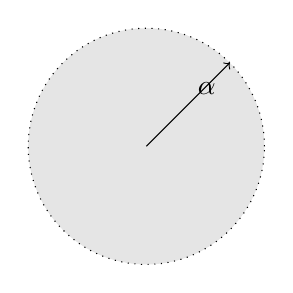
\begin{tikzpicture}
\draw[dotted, fill=gray!20] (0,0) circle (1.5cm);
\draw[->] (0,0) -- (45:1.5cm) node[midway, above right] {$\alpha$};
\end{tikzpicture}

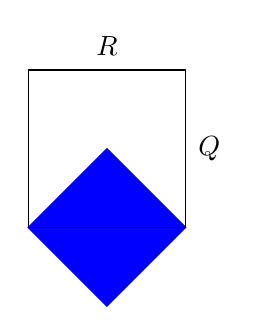
\begin{tikzpicture}
\draw[blue, fill=blue] (0,0) -- (1,1) -- (2,0) -- (1,-1) -- cycle;
\draw (0,0) rectangle (2,2);
\node at (1,2.3) {$R$};
\node at (2.3,1) {$Q$};
\end{tikzpicture}

\end{document}
